% !TEX program = xelatex
\documentclass[12pt]{book}
\usepackage{ctex}
\usepackage{import}
\usepackage{authblk}
\usepackage{amsmath}
\usepackage{graphicx} 
\usepackage{geometry}
\geometry{a4paper,scale=0.8}
\def\celsius{\ensuremath{^\circ\hspace{-0.09em}\mathrm{C}}}
\numberwithin{equation}{section}
\usepackage{tabu}
\usepackage{booktabs}
\usepackage[numbers,sort&compress]{natbib}
\newcommand*{\dif}{\mathop{}\!\mathrm{d}}
\usepackage{caption}
\usepackage[section]{placeins}
\usepackage{float}
\usepackage{placeins}
\DeclareTextFontCommand{\emph}{\bfseries}
\usepackage{verbatim}
\usepackage{amsmath,amssymb}
\usepackage{inputenc}
\usepackage{xeboiboites}
\usepackage{verbatim}
\usepackage{amsmath,amssymb}
\usepackage{braket}
\usepackage{siunitx}
\sisetup{range-phrase = --}
\usepackage{tikz}
\usetikzlibrary{intersections}
\usepackage{pstricks}
\usepackage{makeidx}
\usepackage{subfigure}
%\usepackage{subfig}
\makeindex
%\usepackage{microtype}

%\usepackage{lipsum}
%opening
\title{材料物理}
\author{Wenshan Bai}
\date{\today}

\DeclareTextFontCommand{\emph}{\bfseries}


\newboxedtheorem[
small box style={fill=gray!20,draw=black, rounded corners},
big box style={fill=gray!10,draw=orange,thick,rounded corners},
headfont=\bfseries,
thcounter=section]{define*}{Definition}{}

\newboxedtheorem[
small box style={fill=gray!20,draw=black, rounded corners},
big box style={fill=gray!10,draw=orange,thick,rounded corners},
headfont=\bfseries,
thcounter=subsection]{define}{Definition}{definecounter}

\newbreakabletheorem[small box style={draw=orange,fill=blue!20},
big box style={fill=blue!10,draw=orange}]
{theorem}{Theorem}{theoremcounter}
\newbreakabletheorem[small box style={draw=orange,fill=blue!20},
big box style={fill=blue!30,draw=orange}]
{theorem*}{Theorem}{}
\newbreakabletheorem[small box style={fill=white!20,draw=black, 
	rounded corners},
big box style={fill=white!10,draw=orange,thick,rounded corners},
headfont=\bfseries,
broken edges={draw=orange!30!black!20,thick,fill=orange!20!black!5, 
	decoration={random steps, segment length=.5cm,%
		amplitude=1.3mm},decorate},%
other edges={decoration=penciline,decorate,thick}]%
{example}{Example}{examplecounter}    
\newboxedtheorem[small box style={fill=blue!20,draw=black, 
	rounded corners},
big box style={fill=blue!10,draw=orange,thick,rounded corners},
headfont=\bfseries]%
{example*}{Example}{}  

\newboxedtheorem[small box style={fill=blue!10,draw=black, line width=.7pt,
	decoration={penciline},decorate},%
big box style={fill=blue!10,draw=black,thick, 
	decoration={penciline},decorate},
headfont=\bfseries]%
{Proof}{Proof}{}


\newboxedequation[big box style={fill=blue!10,%
	thick,decoration=penciline,decorate}]%
{formula}      



\newbreakabletheorem[small box style={draw=orange,fill=blue!20},
big box style={fill=blue!10,draw=orange},
broken edges={decoration=zigzag}]
{propd}{Proposition}{test}    

\newbreakabletheorem[small box style={draw=orange!30!black!20,%
	fill=orange!10!black!2,decoration=penciline, decorate, thick},
big box style={color=orange!30!black!20,fill=orange!30!black!10,thick},
broken edges={draw=orange!30!black!20,thick,fill=orange!20!black!5, 
	decoration={random steps, segment length=.5cm,%
		amplitude=1.3mm},decorate},%
other edges={decoration=penciline,decorate,thick}]%
{parchment}{Parchment}{test}    

\newparchment[small box style={draw=orange!30!black!20,%
	fill=orange!10!black!2,decoration=penciline, decorate, thick},
big box style={color=orange!30!black!20,fill=orange!30!black!10,thick},
broken edges={draw=orange!30!black!20,thick,fill=orange!20!black!5, 
	decoration={random steps, segment length=.4cm,%
		amplitude=1.7mm},decorate},%
other edges={decoration=penciline,decorate,thick}]%
{parchmentb}{Parchment}{}     

\newspanning[image=dessins/bulb,headfont=\bfseries,%
spanning style={very thick,decoration=penciline,decorate}]%
{method}{Method}{}

\newspanning[image=dessins/poisson,headfont=\itshape,%
spanning style={very thick,decoration=penciline,decorate}]%
{test}{Test}{}
\usepackage{hyperref}
\hypersetup{
	colorlinks,
	citecolor=black,
	filecolor=black,
	linkcolor=black,
	urlcolor=black
}
%\renewcommand\subfigureautorefname{图}
\renewcommand\figureautorefname{图}
\renewcommand\tableautorefname{表}
\renewcommand\equationautorefname{式}
\usepackage{cleveref}
\begin{document}

\maketitle



\tableofcontents
\addcontentsline{toc}{chapter}{目录}

\clearpage
\chapter*{前言}
	本笔记内容来自材料物理课程材料整理。


\part{晶体缺陷}
	\chapter{点缺陷}
    本部分的内容来自于其他文档,请参考:空位与缺陷.pdf文件。
	\chapter{线缺陷}
    \section{位错概念的引入}
        \subsection{实际晶体的滑移特征}
            在早期对金属材料的范性形变\index{范性形变}的研究中发现:
            \begin{itemize}
                \item[1] 单晶体发生范性形变时表面出现小台阶滑移线;
                \item[2] 晶体滑移总是沿着一定的密排晶面和密排方向,而且只有沿着这些面和方向的切应力达到一个临界值时,滑移才开始进行。
            \end{itemize}
            对与金属单晶来说,这个临界值在\SIrange{1}{10}{\MPa}。在这种情况下,人们引入晶体的理想模型来解决这个问题。

        \subsection{理想晶体的滑移}
            为了解释晶体的变形现象,人们提出了刚性滑移假设\index{刚性滑移假设}。
            假设滑移时滑移面两端的晶体为刚体,原子同步平移,设$T$为加载在晶体上的切应力,在缓慢变形中,该应力与变形相平衡。
            应力大小随滑移面两侧晶体相对位移量变化。

            由于晶体排列具有周期性,点阵对滑移的阻力也是周期性的,变形过程如\autoref{理想晶体变形示意图}所示,
            \begin{figure}[ht]
                \centering
                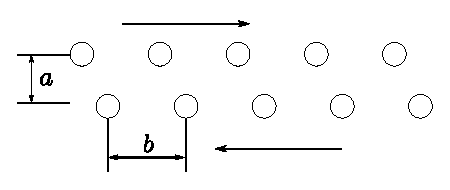
\includegraphics[width=0.7\textwidth]{fig/理想晶体变形示意图.eps}
                \caption{理想晶体变形示意图。}
                \label{理想晶体变形示意图}
            \end{figure}
            
            假定变形所受到的阻力为
            \begin{equation}
                \tau=\tau_m\sin{\left( \frac{2\pi x}{b} \right)}
            \end{equation}
            当发生的变形很小时,可以近似为
            \begin{equation}
                \tau=\tau_m{\left( \frac{2\pi x}{b} \right)},
            \end{equation}
            而且开始变形时,晶体处于弹性阶段,应当满足虎克定律,也就是
            \begin{equation}
                \tau=\mu\gamma=\mu\frac{x}{a},
            \end{equation}
            其中$\mu$为切变模量,$\gamma$为切应变,因此可以得到最大切应力为
            \begin{equation}
                \tau_m=\frac{\mu b}{2\pi a},
            \end{equation}
            由于本课程讨论的晶体绝大多数情况为简单立方晶系,可以认为$a=b$,所以最大切应变为
            \begin{equation}
                \tau_m=\frac{\mu}{2\pi}.
            \end{equation}

            然而理论切变强度$\frac{\mu}{2\pi}$与实际强度相比,实在太大。在使用更为合适的原子间作用力模型后,改变了正弦近似,
            最大切应变数值上降低为原来的$1/60$,但是这仍然比实际值高出了3到4个数量级。

            然而无论如何都提高应力模型的精确程度,最终结果的偏差仍然很大,因此是假设出现了问题。最终人们提出了位错模型,并且在
            实验中观察到了这一现象。
        
    \section{位错的结构}
        晶体中存在三种不同的位错类型,下面将分别描述。
            \subsection{刃型位错}
                考虑一个简单立方晶体,它在$(010)$面上沿$[100]$方向发生滑移,但是这个滑移是不均匀的。
                也就是从晶体的右侧向左传播。在某一时刻,滑移停止在晶体内部。于是在这个$(010)$面左右就可以划分出已滑移区域和未滑移区域,
                该面也就是两个区域的边界。晶体滑移的元过程是在一定的晶体学面上,沿一定的晶体学方向,晶体的上下两部分相对滑移一个或着多个
                点阵常数的距离。

                由此显然可见,已滑移的地区与未滑移的地区是一样的,上述滑移平面上下原子列是恢复对齐的,也就是说,这些地方恢复了理想晶体的长程
                有序性。所以除去\autoref{刃型位错形成示意图}中$\perp$的位置外,晶体的其他部分都是完整的。在这一区域内,晶体的完整周期性显然被
                破坏,所以这就是一个晶体缺陷,称为位错\index{位错}。
                \begin{figure}[ht]
                    \centering
                    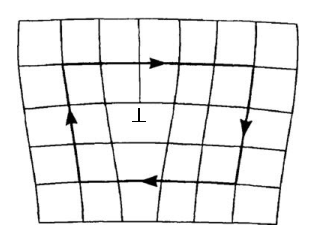
\includegraphics[width=0.45\textwidth]{fig/刃型位错示意图b.eps}
                    \caption{刃型位错形成示意图。}
                    \label{刃型位错形成示意图}
                \end{figure}

                关于位错最为简单的定义就是:位错是近完整晶体中的一个缺陷,是晶体中已滑移区和未滑移区的边界。
                
                这个边界更为严格的说,是分界区域的中心轴线,是平行于$[011]$方向的一条直线,其与滑移矢量$[100]$垂直,那么
                这个位错就称为刃型位错。

                上述中心轴线称为位错线\index{位错线},原理位错线的区域保持理想晶体的完整性;只有极为接近位错线的区域,也就是上述分界区域或
                过渡区域,晶体的点阵结构,或者原子的规则排列被破坏这一区域称为位错核心\index{位错!位错核心}。位错核心的半径与位错线的长度
                相比非常小,所以说,位错是晶体中的线性缺陷。

                对于刃型位错\index{位错!刃型位错},其与滑移矢量垂直,而\autoref{刃型位错形成示意图}中,$\perp$符号代表多余的一个半原子面,
                这个半原子面的边缘就是刃型位错的位错线,形状类似刀刃,因此称为刃位错\index{位错!刃位错}。
                因此刃型位错的形成也可以认为是一个半原子面中断与晶体内部,该边缘也就是一个刃型位错。

                在规定分割面的上下后,半原子面在割面上方的位错称为正刃型位错,反之则为负刃型位错,但是两者并没有本质上的区别。

                刃型位错有以下结构特点
                \begin{itemize}
                    \item[1] 位错周围有弹性畸变或非弹性畸变,上半部分晶体受压力,下部分受张力,中心为最大畸变,畸变局限在2或3个原子间距的管道内,总体为线缺陷;
                    \item[2] 位错线与滑移方向垂直;
                    \item[3] 上下晶体有一个相对位移$\vec{b}$,称为伯格斯矢量或简称柏式矢量\index{柏式矢量}。
                \end{itemize}
            \subsection{螺型位错}
                仍然假定滑移面为$\left( 010 \right)$面,位错线仍然是沿$[001]$方向的直线,但是滑移方向变为$[001]$方向,
                即为与位错线平行的方向,仍然将晶体分为已滑移区、未滑移区以及中间的过渡地带。同样,整个晶体是近完整的,只有在位错核心区,晶体的点阵
                结构才遭到破坏。
                
                也就是说,这也是一个二维缺陷,但是原子排列方式与刃型位错却不相同,不难得出,对与位错线垂直的原子面
                在位错不存在时,是一组彼此平行分立的平面,当此位错存在时,他们则变成一个连续的螺旋面。
                若绕此位错线以左手螺旋正向环行一周,即从一个面上升到相邻的另一个原子面,由于这个形质,这种位错称为螺型位错\index{位错!螺位错}。
                
                \begin{figure}[ht]
                    \centering
                    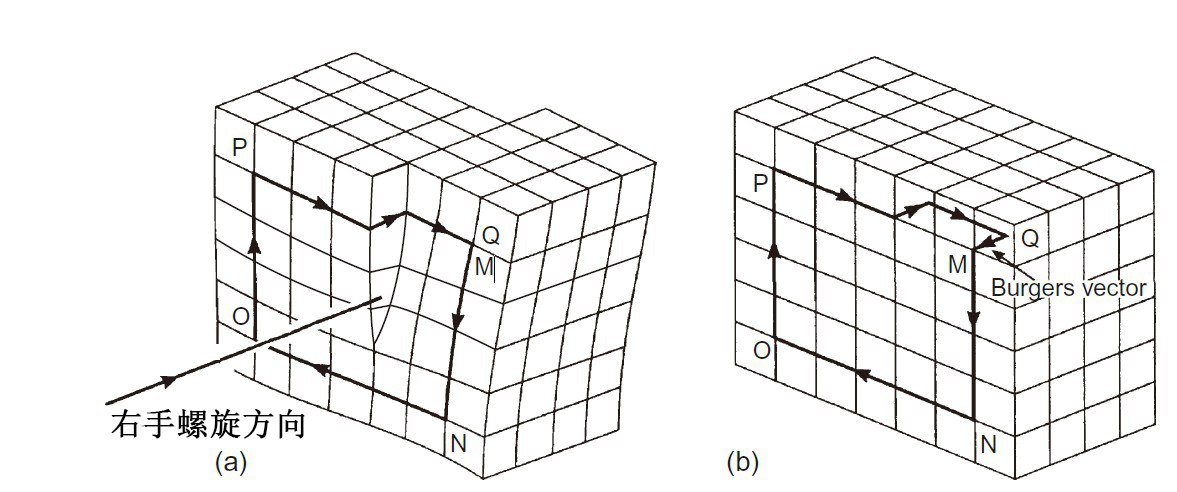
\includegraphics[width=0.7\textwidth]{fig/螺型位错示意图.jpg}
                    \caption{左螺型位错示意图,(a)螺型位错的左手螺旋回路,(b)为相同回路在理想晶体中的绕行状况。}
                    \label{螺型位错示意图}
                \end{figure}

                在规定位错线正方向后,若绕位错线以右手螺旋方向绕行一周后,可以上升一个原子面的位错为右螺型位错,
                若绕位错线以左手螺旋方向绕行一周后,可以上升一个原子面的位错为左螺型位错,如\autoref{螺型位错示意图}。
                左螺型位错和右螺型位错的滑移矢量方向也是相反的。

                在含有螺型位错的晶体中,原子面排布如\autoref{右螺型位错原子面排布}所示。晶体不再是刃型位错的附加半原子面,而是变成了螺旋式的曲面。
                \begin{figure}[ht]
                    \centering
                    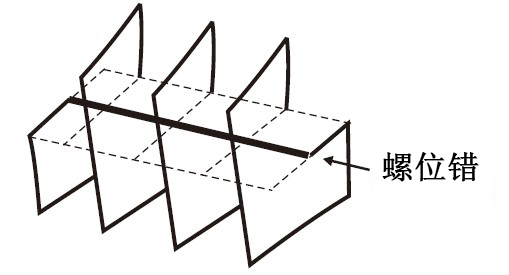
\includegraphics[width=0.5\textwidth]{fig/螺位错原子面排布.jpg}
                    \caption{右螺型位错原子面排布。}
                    \label{右螺型位错原子面排布}
                \end{figure}
            \subsection{混合型位错}
                然而一根直线位错可能既不与滑移矢量$\vec{b}$垂直,也不平行,而是成一个角度$\theta$,则这个位错既不是纯刃型位错也不是纯螺型位错,
                它可以看作是两个直线位错的叠加,分别为纯刃型和纯螺型的位错,两者的滑移矢量大小为
                \begin{align}
                    \vec{b}_1&=\vec{b}\sin\theta,\\
                    \vec{b}_2&=\vec{b}\cos\theta.
                \end{align}
                这个直线位错称为混合位错\index{位错!混合位错}。组成混合位错的两个分量为刃型分量和螺型分量。

                对上述情况加以推广,假设滑移矢量为$\vec{b}$,已滑移区域为\autoref{混合型位错的滑移示意}中的阴影部分,而位错线为图中红色线,从垂直与滑移面的方向看去,上下两个原子
                面之间的原子排布应该为\autoref{混合型位错的原子排列示意图}所示。
                \begin{figure}[ht]
                    \centering
                    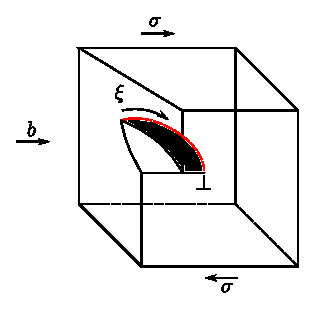
\includegraphics[width=0.5\textwidth]{fig/混合型位错的滑移示意.eps}
                    \caption{混合型位错的滑移示意。}
                    \label{混合型位错的滑移示意}
                \end{figure}
                
                \begin{figure}[ht]
                    \centering
                    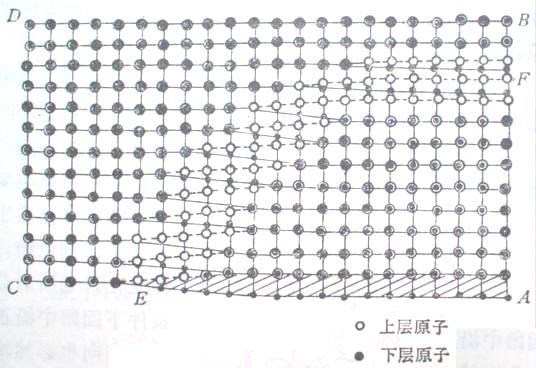
\includegraphics[width=0.5\textwidth]{fig/混合型位错的原子排列示意图.jpg}
                    \caption{混合型位错的原子排列示意图。}
                    \label{混合型位错的原子排列示意图}
                \end{figure}
                从\autoref{混合型位错的原子排列示意图}可以看出,这个位错有一段是纯螺型位错,另一端是纯刃型位错,由于位错线是连续的\footnote{这一点需要会证明。}
                从晶体的一个表面延伸到另一个表面,中间弯曲的一端既不是螺型位错也不是刃型位错,而是同时具有螺型和刃型位错的特征。
                这一小段也可以看作是许多方向近连续变化的小直线段所组成,每一小段都是混合型位错,各有一个螺型分量和刃型分量。
            \subsection{小结}
                依照以上定义,位错是晶体中滑移面上两个区域(即已滑移区域和未滑移区域)之间的分界,那么它就应该具有两个重要的性质:
                \begin{itemize}
                    \item[1] 因为晶体的滑移矢量是一个恒定矢量,等于一个或多个最小点阵平移矢量,所以对于一条位错线的各个部分,滑移矢量均相等;
                    \item[2] 无论位错线形状如何,总之位错线绝不可能终止于晶体的内部,位错线只能从晶体的一个表面延伸到另一个表面,或是在晶体中形成一个封闭的环。
                \end{itemize}
        \section{位错的普遍定义与伯格斯矢量}\label{section:位错的普遍定义与伯格斯矢量}
            \subsection{位错的普遍定义}
                在直观的基础上对位错的几何性质有一定的了解以后,我们这里可以对位错作出更为普遍的定义。

                假设晶体沿任意面$S$剖开,将$S$面的两边$S_1$以及$S_2$作一刚性的相对位移$\vec{b}$,$\vec{b}$可以是
                晶体中任意的电子平移矢量\footnote{$\vec{b}$不是点阵矢量的情形将在以后做出讨论。},经过这样的操作以后,
                如果$\vec{b}$与$S$面不平行,有些地方将产生原子位置重叠或者是空隙。去掉重叠的原子,空隙按照晶格排列填补,
                这样$S$面不会有任何改变,但是晶体中出现相对位移和未相对位移区域的分界线,也就是$S$面的周界。在分界线上原子错排的情况就是
                位错线\index{位错线},$\vec{b}$为伯格斯矢量或柏式矢量\index{柏式矢量},其为位错特征的标志,数值大小为$b$,
                称为位错的强度\index{位错!强度}。

                晶体中任意的位错都可以按照上面操作来形成, 但是汽油有一些需要注意的地方:
                \begin{itemize}
                    \item[1] 上述的想象操作不仅是用来说明位错的特征,也模拟了晶体产生位错的实际过程,关于位错生成的过程将以后讨论;
                    \item[2] 对于同一根位错线,可以有不同的$S$面,只要柏式矢量相图,形成的就是相同的位错,因此决定位错特征的是伯格斯矢量,而不是$S$面的具体位置,可以选以位错为边界的任意面作为上述操作的$S$面,比如沿$z$轴的刃型位错,选取$xoz$面和$yoz$面的结果是一致的;
                    \item[3] 实际上,从已经做过相对位移的区域到未作相对位移的区域间的过渡不可能是突变的,否则将产生无法填补的裂缝,因此$S$面两侧的刚性位移在边界是不再适用的,准确到说,位错不是一根线,而是有一定宽度$w$的区域,在这个区域内,$b$从中心的最大值下降到边界的零,只是由于宽度比长度小得多,所以可以近似为一根线。
                \end{itemize}
    
                \subsection{柏式矢量的定义}
                    $\vec{b}$矢量称为柏式矢量,它是位错线特征的标志,位错的强度为$b$,而方向的确定常使用伯格斯回路法和Frank惯例法。
                    \subsubsection{伯格斯回路法}
                        实现选取有位错的实际晶体,从好区中任意原子出发,微扰位错作一个闭合回路,回路每一步都连接相邻的同类原子,并且始终走在晶体的好区,这个回路称为伯格斯回路\index{伯格斯回路}。
                        然后在完整晶体中作一个对应的回路,即在相同方向走相同步数,结果发现这个回路无法闭合。终点到起点的矢量$\vec{b}$为柏式矢量\index{柏式矢量},回路
                        的方向与位错线方向成右手螺旋的方向为正方向。

                        假设晶体中三个基矢量$\vec{a}_0$,$\vec{b}_0$,$\vec{c}_0$,整个晶体的矢量都可以使用这三个矢量表示。
                        在理想晶体中,绕行晶体一周后必然有
                        \begin{equation}
                            \sum_{a}n_a\vec{a}_0+\sum_{c}n_b\vec{b}_0+\sum_{c}n_c\vec{c}_0=0\label{完整晶体的绕行结果},
                        \end{equation}
                        其中$n$为整数。

                        假如晶体不是完善的而是含有点缺陷,\autoref{完整晶体的绕行结果}仍然成立,但是基矢量在不同地方的长度有弹性范围内的差异,
                        这是因为点缺陷附近有弹性畸变,离开点缺陷稍远的地方,弹性畸变相应减少。

                        加入这个封闭回路本身经过的地方都是良好的,但是回路包围的区域中含有一个位错$\vec{b}$,回路的方向与位错的方向构成右手螺旋关系,对这个回路,\autoref{完整晶体的绕行结果}变为
                        \begin{equation}
                            \sum_{a}n_a\vec{a}_0+\sum_{c}n_b\vec{b}_0+\sum_{c}n_c\vec{c}_0=-\vec{b},                            
                        \end{equation}

                    \subsubsection{Frank惯例法}
                        Frank惯例法\index{Frank惯例法}需要线确定位错线的正向,割面及割面法线的正向,按照右手螺旋定则,四个手指顺位错线垂直防御割面上,大拇指指向正半晶体也就是法线方向,规定$\vec{b}$为
                        负半晶体相对与正半晶体的移动方向。

                        在确定$\vec{b}$后,如果位错线与$\vec{b}$平行,则为螺旋位错,方向相同为正,反向为负;如果$\vec{b}$与位错线垂直,
                        则为刃型位错,对于刃型位错的方向,需要使用半原子面右手法,如\autoref{刃型位错的半原子面右手法则}所示。
                        \begin{figure}[ht]
                            \centering
                            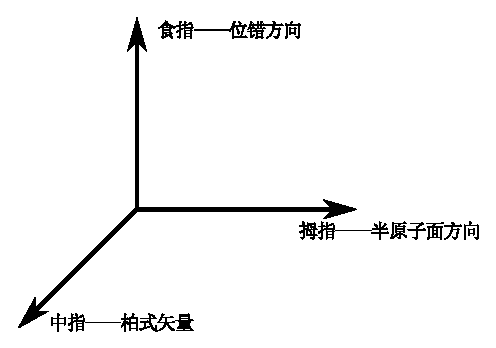
\includegraphics[scale=1]{fig/刃型位错的半原子面右手法则.eps}
                            \caption{刃型位错的半原子面右手法则。}
                            \label{刃型位错的半原子面右手法则}
                        \end{figure}
                \subsection{柏式矢量守恒定律}
                        利用柏式回路的概念即可论证伯格斯矢量的守恒定律:
                        \begin{enumerate}
                            \item[1] 一个位错线不可能中止于晶体内部,它必然构成闭合1的圈或终止于晶体表面,沿一根不分岔的位错线的伯格斯矢量是守恒的,具有相图的大小和方向。
                            \item[2] 如果数根位错线相较于一点,此点称为位错的节点\index{节点},朝向节点的各位错线柏式矢量的总和等于流出各节点位错线伯格斯矢量矢量的总和,如果所有的位错线方向都是从节点出发,则上述关系可以写作各分支柏式矢量的总和为零,即$\sum b=0$;
                            \item[3] 柏式回路有如下特点:
                            \begin{enumerate}
                                \item[1)] 一根位错线只有一个柏式矢量;
                                \item[2)] 位错线不能在晶体内部中断,因而它们只能或者终止在晶体表面,或者形成封闭环,或者与其它位错相联;
                                \item[3)] 当位错与其它位错相联时,指向结点的位错柏氏矢量和与离开节点位错的柏氏矢量和相等,若均指向一个节点,有$\sum b=0$。
                            \end{enumerate} 
                        \end{enumerate}
        
        \section{位错应力场}
            根据\autoref{section:位错的普遍定义与伯格斯矢量},位错是一个线缺陷,其最大畸变分布在以位错线为轴心的管道区域内,管道的直径为2到3个原子间距。
            同时位错的畸变与距离位错线的距离成反比,距离越远的区域,畸变也越小。
        \section{位错的应变能}
        \section{位错的线张力}
        \section{位错核心}
        \section{位错的受力与运动}
        \section{位错与晶体缺陷间的相互作用}
        \section{位错的增殖}
        \section{实际晶体中的位错}
        
	\chapter{晶粒边界}
    多晶体材料中,多个晶粒在凝固时的方向不同,因此在边界处的排列方式需要研究,将两个晶粒之间的边界称为晶界\index{晶界}。
    它是把结构相同但相位不同的两个晶粒分隔开的面状晶格缺陷,是本课程中除了层错以外的另一种面缺陷。

    如果吧晶界看作两个晶粒由于取向差的不同造成了晶界,可以发现,界面在空间的方程有2个自由度,而取向差可以认为是有一个晶粒相对与另一个晶粒进行了旋转,这样,可以说
    旋转轴这条直线的方程中有2个自由度,最后旋转角度为第5个自由度:
    \begin{itemize}
        \item[1] 位相差$\theta$;
        \item[2] 发生位相差$\theta$的转动轴的方向余弦,其中仅有两个是独立的量;
        \item[3]  晶界面法线的方向余弦(其中任意二个),这个方向是用来表示晶界在空间取向的。 
    \end{itemize}
    概括起来,就是产生位相差的转动角$\theta$,表示转动轴上单位矢量$\vec{U}$方位的两个参数以及表示晶界发现单位矢量$n$的两个参数。
    假如直到了这些参变量和晶型,就可以确定晶界的位错模型。
    \section{晶界结构}
        一组平行排列的直的刃型位错的稳定平衡位置是沿$y$轴成了一条直线排列,形成位错墙,而形成这一位错墙的原因是墙的两侧有着较大的取向差。
        \subsection{小角度晶界}
            简单晶界有两种类型:倾斜晶界和扭转晶界。设$U$是发生位相差的相对旋转轴上的单位矢量,$n$是晶界面法线上的单位矢量,则纯粹倾转晶界的条件是    
            \begin{equation}
                U\cdot n=0,
            \end{equation}
            如果晶界面与产生取向差的旋转轴垂直,即$U\parallel n$,就构成了简单的扭转晶界。
            \subsubsection{倾转晶界}
                假设两个简单立方晶体具有相同的$[001]$轴,它们之间的位向差是绕着共同轴相对转动$\theta$角而产生的,两个晶粒的截面是一个对称面,
                都和$(100)$面平行。两个晶体以这种方式连接必然导致连接区域的畸变,而且弹性变形区将扩展到足以松弛晶界的应力集中。除了弹性形变还需要一些竖直
                的原子面终止在晶界上,形成刃型位错,其柏式矢量基本都是$[100]$平移矢量,而柏式矢量$\vec{b}$、位错间距$D$和位相差$\theta$的关系为:
                \begin{equation}
                    \frac{b}{D}=\theta,
                \end{equation}
                当$\theta$小于\ang{15}时,为小角晶界,大于\ang{15}时,为大角晶界。
            \subsubsection{扭转晶界}
        \subsection{大角度晶界}
            对于大角晶界仍然没有得到完美的研究结果,此处主要介绍当前的研究进展。

            过冷液体模型认为大叫晶界是几层原子排雷而成,与过冷液体类似,呈非晶态。但是过冷液体在热力学上不稳定,而晶界存在符合平衡条件。
            另外这一模型认为晶界层上将有两个固液界面,这是不能实现的。

            之后又提出了小岛模型等,都不能解释晶界结构。目前较为有效的模型有重合位置电子模型(CSL),假设一下特殊位向的晶界中,有一些原子同属于两边晶粒的格点,
            并自身形成超格点点阵。模型认为大角晶界由约两原子直径厚的对拍和错排区后才,重合位置点阵和大角晶界的关系:
            \begin{itemize}
                \item[1] 重合关系只出现在某些特定的晶界上,晶界总处于重合点阵的最密排面上,而且能量最低厚度很小,长程应变场可以忽略不计;
                \item[2] 晶界与重合电子的最密排面间有一个小角度时,为了使晶界在重合点阵的最密排面上有最大的面积起见,便会产生阶。阶也不具有长程应变场,但如果在晶界上加一适当的应力,它可能成为位错的增殖源;
                \item[3] 与理想重合位置位向稍有偏离的晶界,可以用一个重合位置晶界同一与它在同一平面上的晶界位错网络叠加在一起来描述。一般这种晶界位错的柏氏矢量较晶格位错的为小,故有次位错之称。
            \end{itemize}

            后来又提出了O点阵的概念,O点阵的结点是指在点上看各自晶格近邻关系是相同的,只差一个转角的点,不一定是原子占据的点。
    \section{晶界能量}
        晶界能量来源于两个晶粒边界上很多原子从晶格的正常位置移动出来,并且在附近晶体中引起畸变。我们定义单位面积所对应的能量增加量为晶界能量\index{晶界能量}。
        \subsection{小角度晶界的能量}
            在晶界的各种性质中,晶界能是很重要的物理量,目前关于小角晶界能的计算有
            很多方法。下面介绍一种简明近似的方法,以对称倾斜晶界为例。单位长度位错的能量为:
            \begin{equation}
                W=\frac{\mu b^{2}}{4 \pi(1-v)} \ln \left(\frac{r_{1}}{r_{0}}\right)+W_{A B},
            \end{equation}
            其中,$W_{AB}$为刃型位错中心能,$r_1$为位错弹性应力场所及的距离,大小为亚晶尺寸,$r_0$为位错核心区。

            在单位长度内的位错数量为$1/D$,$D$为位错间距,
            根据
            \begin{equation}
                \frac{1}{D}=\frac{\theta}{b},
            \end{equation}
            另$b=r_0$,$r_1=D$,位错的能量可以写作
            \begin{equation}
                \begin{split}
                    W&=\frac{\theta}{b}\left[\frac{\mu b^{2}}{4 \pi(1-v)} \ln \left(\frac{1}{\theta}\right)+W_{A B}\right]\\
                    &=\frac{\mu b \theta}{4 \pi(1-v)} \ln \left(\frac{1}{\theta}\right)+\frac{\theta}{b} W_{A B}\\
                    &=E_{0} \theta[A-\ln \theta],
                \end{split}
            \end{equation}
            
        \subsection{大角度晶界的能量}
            由于大角晶界结构未知,可以使用测量的方法,假设三个晶界相较于一个公共的交线,平衡的条件为
            \begin{equation}
                \mathrm{E}_{1} / \sin \psi_{1=} \mathrm{E}_{2} / \sin \psi_{2}=\mathrm{E}_{3} / \sin \psi_{3};
            \end{equation}
            一般测量时习惯将两大角晶界能当作不变的参值,而改变第三晶界的旋转角。
            也可用表面沟槽法,表面张力为
    \section{晶界的运动}
        \subsection{小角晶界的移动}
            晶界的应力感生迁移,晶界受到的力为
            \begin{equation}
                P=\tau\cdot b=\theta\cdot\tau,
            \end{equation}
            晶界的迁移率为$B$,驱动力$F$,则迁移速度为
            \begin{equation}
                v=F\cdot B,
            \end{equation}
            驱动力
            \begin{equation}
                F=\frac{\dif \mu}{\dif x},
            \end{equation}
            也就是反化学位梯度的方向\footnote{扩散中原子的运动的方向为化学位的梯度方向}。
            

\part{性能强化}
	\chapter{晶体的范性变形}
    \section{单晶体的滑移变形}
        \subsection{滑移晶体学特征}
        \subsection{影响滑移系统的因素}
        \subsection{滑移方式与滑移带}
    \section{单晶体屈服与晶体的转动及碎化}
        \subsection{临界分切应力定律}
        \subsection{临界切应力的位错理论}
            晶体收到外应力作用,取向因子最大的滑移系位错开始滑移,其他位错或晶体缺陷要对它的运动产生
            阻碍或交互作用,主要考虑以下几种
            \begin{enumerate}
                \item[1] 位错增殖;
                \item[2] 点阵阻力;
                \item[3] 与其他位错的交互作用:
                \begin{enumerate}
                    \item[1] 弹性应力场的交互作用。为了简便起见,设有二个位错排列在垂直的方向,相距为l。位错要从B、C中间穿过去,就要克服B、C的长程弹性作用力。假设平行于可动位错的那些位错均匀分布,这些位错之间的间距用$l_1$表示,可以推导得出:位错克服的应力为$\tau=\alpha\mu b\sqrt{\rho}$。
                    \item[2] 位错塞积;塞积导致应力集中\footnote{如果塞积群与所求位错之间距离较远,可以视塞积群为一个扩大$N$倍的柏式矢量,其中$N$为塞积群位错数量。}。位错受到的阻力为$\tau_0^2=\alpha\frac{\mu b}{l_2}$
                    \item[3] 位错绕过位错林;与增殖过程相似,在林位错周围形成位错环,然后继续滑移,阻碍切应力为$\tau_0^3=\alpha\frac{\mu b}{l_2}$;
                    \item[4] 以上的三个$\alpha$并非同一常数,仅仅为方便使用同一符号,而且以上的阻力与位错的温度没有关系,
                    \item[5] 切过林位错产生交割,这一部分是短程相互作用,与热激活有关,这是温度升高,屈服强度降低的原因。外力为$\tau$,长程应力为$\tau_0$,外力完成完全切割做功为$W=(\tau-\tau_0)bld$,产生割阶的能量为$\Delta H_0$,热激活提供的能量为$\Delta H=\Delta H_0-(\tau-\tau_0)bld$,当温度高于一定值,形成割阶的能量完全由热激活提供,不需要外力。
                \end{enumerate} 
            \end{enumerate}
            提高屈服强度也就是提高位错运动的长程和短程阻力,主要有以下途径:
            \begin{itemize}
                \item[1] 位错密度上升,比如通过拉拔进行加工硬化,桥梁钢在处理后屈服强度可提升50\%;
                \item[2] 障碍物尺寸增加;
                \item[3] 障碍物间距缩小,也就是增加障碍物密度,比如弥散强化;
                \item[4] 障碍物的稳定性增加。
            \end{itemize}
            影响临界分切应力$\tau_0$的因素
            \begin{itemize}
                \item[1] 高温段不发生变化,温度降低,应力上升,对韧性产生影响;
                \item[2] 合金元素的存在,一般会使临界切应力$\tau_0$增加;
                \item[3] 应变使位错密度增加,进而也会使切应力增加;
            \end{itemize}
        \subsection{拉伸过程中集体的转动和碎化}
            滑移面与拉伸轴不平行,切变方向沿滑移方向,无法沿拉伸轴方向,因此,试样两端会产生位移。在拉伸实验中,两端被限制,晶面会受到转动力矩的作用,从而发生转动。

            在不能整体发生倾转的时候,表面出现$S$状的滑移线,同号的位错堆积起来,然后产生晶体弯曲,变形过程中晶体的碎化,在取向差小于\ang{15}时\footnote{小角晶界处。},将会出现亚晶。
            产生畸变后,在衍射斑上会出现星芒。
        \subsection{孪生}
            孪生是晶体塑性变形的另一种方式,比如,体心立方的金属的六个偏位错滑移产生孪晶,当晶体的一部分相对另一部分呈镜面对称时,两者互为孪晶。
            
            其与滑移的差异
            \begin{itemize}
                \item[1] 原子到孪生面的移动距离不是常数;
                \item[2] 抛光之后仍然可见;而滑移是表面现象,内部不产生畸变,而孪生不会因为抛光改变晶体排列,仍然可见;
                \item[3] 形状通常为薄透镜状;
                \item[4] 发生速度可以很快;
                \item[5] 一般是滑移受阻时产生的。
            \end{itemize}
        \subsection{总结}
            单晶体塑性变形的三个过程:1.切变,2.转动,3.碎化。
    \section{多晶体范性变形的特点及晶界的作用}
        \subsection{多晶体塑性变形的特点}
            一般情况下,多晶材料屈服应力大于单晶材料,因为晶界会产生强化效应。
            在若干晶系中,选择$\omega$最大的取向最先发生开动,晶粒中发生多滑移,使其发生变形的方向一致。二这需要至少五个滑移系同时运动。
            这也是多晶变形的特点之一:多滑移。

            在晶界附近,为位错滑移受到阻碍,发生位错塞积。

            在变形过程中,会出现择优取向,也就是织构。
        \subsection{多晶体的屈服应力}
            假设在A 晶粒中的某个滑移系处于有利的取向,其取向因子最大,也最先开始滑
            移,滑移后位错遇到晶界,位错塞积,之后在B晶粒的晶界处产生应力集中,当应力集中过大时,
            B中的滑移系达到了临界应力,也会发生滑移,变形也就从$A$传递到了$B$。这是变形的传递过程。

            假设A晶粒中的变形可以表示为
            \begin{equation}
                \gamma=\frac{nb}{L},
            \end{equation}
            其中$L$为A晶粒的滑移方向的长度,
            此时B晶粒没有发生位错滑移,仍然处于弹性变形阶段,所以

\part{固溶体、扩散与相变}
	\chapter{固溶体}
	\chapter{扩散}
	\chapter{相变}
    \section{相变概念}
        关于相变,有一些最为基础的概念,
        \begin{enumerate}
            \item 相\index{相}:成分相同、结构相同,有界面同其他部分分隔的物质均匀组成部分;
            \item 相变\index{相变}:当外界条件(如温度、压力等)连续变化时,物质自身发生突变的现象。或物相的某个(阶)热力学势跃变,伴随物相的某个(些)要素跃变;
            \item 固态相变\index{固态相变}:固体材料的结构在温度、压力、成分改变时所发生的转变。
        \end{enumerate}

        在分类上,有很多种分类方法,比如从动力学上,或者是从热力学上分类
            \subsection{动力学相变分类}
                相变分为两类:扩散性和无扩散型,如\autoref{金属及合金中的一级相变}所示。
                无扩散型相变\index{无扩散型相变}较为简单,分为连续型相变\index{连续型相变},比如$\omega$相比\index{$\omega$相变},和形核长大型相变\index{形核长大型相变},比如马氏体相变\index{马氏体相变}。

                而扩散性相变\index{扩散性相变}则相对复杂,也分为连续型相变\index{连续型相变}和形核长大型相变\index{形核长大型相变},更为具体的分类将在后面的章节进行讲解,在这里不再进行过多叙述。
                \begin{figure}[ht]
                    \centering
                    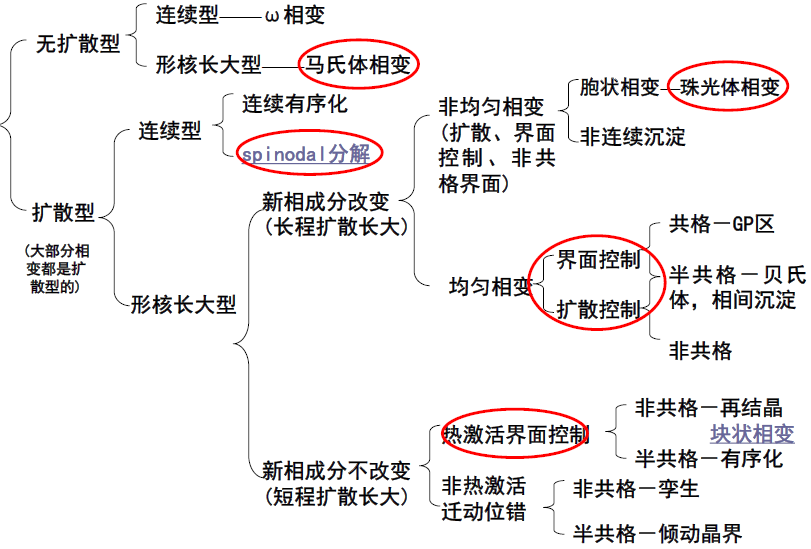
\includegraphics[width=0.7\textwidth]{fig/金属及合金中的一级相变.png}
                    \caption{金属及合金中的一级相变。}
                    \label{金属及合金中的一级相变}
                \end{figure}
            \subsection{热力学的相变分类}
                在热力学的分类比较简单,分为一级相变\index{一级相变}和二级相变\index{二级相变}。
                一级相变是指化学位相等,但是化学位的一阶导数不等,也就是熵不等或者是体积不等,
                \begin{align}
                    \mu_1&=\mu_2,\\
                    \left(  \frac{\partial\mu_1}{\partial T} \right)_p=-S_1&\neq-S_2= \left(  \frac{\partial\mu_2}{\partial T} \right)_p\label{等压一级相变},\\
                    \left(  \frac{\partial\mu_1}{\partial p} \right)_T=V_1&\neq V_2= \left(  \frac{\partial\mu_2}{\partial p} \right)_T\label{等温一级相变}.
                \end{align}
                在一级相变中伴有能量变化,或者吸热或者放热,或者体积发生变化。比如晶体的熔化、升华、液体的凝固、汽化、气体的凝聚以及晶体中大多数晶型转变都属于一级相变,这是最普遍的相变类型。

                二级相变是指化学位的二阶导数发生突变,而化学位和一阶导数不发生突变,
                \begin{align}
                    -\frac{C_p}{T}=\left(  \frac{ \partial^2\mu_1  }{\partial T^2} \right)_p&\neq\left(  \frac{ \partial^2\mu_2  }{\partial T^2} \right)_p,\\
                    kV=\left(  \frac{ \partial^2\mu_1  }{\partial p^2} \right)_T&\neq\left(  \frac{ \partial^2\mu_2  }{\partial p^2} \right)_T,\\
                    \alpha V=\frac{\partial^2\mu_1}{\partial T\partial p}&\neq\frac{\partial^2\mu_2}{\partial T\partial p}.
                \end{align}
                其中$C_p$为等压比热\index{等压比热},$k$为等温等压系数\index{等温等压系数},$\alpha$为等压膨胀系数\index{等压膨胀系数}\footnote{熔化、马氏体转变属一级相变,有序化可能是一级也
                可能是二级相变。}。
                在二级相变中,两相的化学势、熵和体积相等,但热容、膨胀系数和压缩系数不相等,即无相变潜热,无体积的突变,只有热容、
                膨胀系数和压缩系数的不连续变化,
                \begin{align*}
                    \Delta C_p\neq 0,\\
                    \Delta\beta\neq 0,\\
                    \Delta\alpha\neq0.\\
                \end{align*}
                一般合金的有序-无序转变、铁磁-顺磁转变、超导转变等属于二级相变。大多数便随某种物理性能的变化。
            \subsection{固溶体自由能的计算}
                纯组元的自由能和温度的关系可以写作
                \begin{equation}
                    G(T)=H(T)-TS(T),
                \end{equation}
                而两相混合的自由能,在理想条件下可以由两相的自由能叠加得到。

                假设在体系中存在两种相$\alpha$和$\beta$,均是由A、B两种原子构成,假设A原子的成分为$x\mathrm{at.}\%$,在$\alpha$相中,A的原子百分比为$x_1$,在$\beta$中的原子百分比为$x_2$
                而$\alpha$相和$\beta$的占比分别为$N_1$和$N_2$,两者的自由能分别为$G_1$和$G_2$,混合后的自由能为
                \begin{equation}
                    G=N_1G_1+N_2G_2,
                \end{equation}
                利用成分关系,可以变为
                \begin{equation}
                    G=G_1+\frac{x-x_1}{x_2-x_1}(G_2-G_1),
                \end{equation}
                所以$G_1$,$G$,$G_2$处于同一直线,并且服从杠杆定律。

                但是在混合过程存在其他作用,导致混合后的自由能不等于理想情况下的自由能。这里假设实际的自由能为
                \begin{equation}
                    G(x)=G^0+\Delta G^m,
                \end{equation}
                其中
                \begin{equation}
                    G^0=x_AG_A^0+x_BG_B^0,
                \end{equation}
                其中,$x_A$为$A$原子的原子百分比,$x_B$为$B$原子的原子百分比,而要计算$\Delta G^m$,需要先计算混合过程中的焓\index{焓}和熵\index{熵}的变化量。
                \subsubsection{混合过程中熵的改变量}
                    固态下的系统的熵主要由混合熵\index{熵!混合熵}(决定于原子可能排列的方式)和振动熵\index{熵!振动熵}(决定于温度和缺陷)组成,
                    混合熵的变化为
                    \begin{equation}
                        \Delta S^m=S_{AB}-(x_AS_A+x_BS_B),
                    \end{equation}
                    根据混合熵的定义
                    \begin{equation}
                        S=k\ln{\Omega},
                    \end{equation}
                    其中$k$为玻尔兹曼常数,$\Omega$为微观状态数,假设$A$的原子数为$N_A$,$B$的原子数为$N_B$,混合熵的变化为
                    \begin{equation}
                        \begin{split}
                        \Delta S^m&=S_{AB}-(x_AS_A+x_BS_B)\\
                        &=k\ln{\frac{N!}{N_A!(N-N_A)!}}-x_Ak \ln \left(C_{N_{A}}^{N_{A}}\right)  -x_Bk \ln \left(C_{N_{B}}^{N_{B}}\right)\\
                        &=k\ln{\frac{N!}{N_A!N_B!}}\\
                        &=k\left( \ln{N!}-\ln{N_A!}-\ln{N_B!} \right).                
                        \end{split}                                      
                    \end{equation}
                    根据Stirling公式,
                    \begin{equation}
                        \Delta S^m=-R(x_A\ln{x_A}+x_B\ln{x_B}),
                    \end{equation}
                    其中$R=kN$。
                \subsubsection{混合过程中焓的改变量}
                    接下来计算混合过程中焓的变化,利用溶液的准化学模型\index{准化学模型},假设
                    \begin{enumerate}
                        \item $A$,$B$两组元尺寸接近,排列无序;
                        \item 混合过程中体积基本不变,即$\Delta V=0$;
                        \item 原子只与最近邻的原子之间存在相互作用,即只计算最近邻原子之间的结合能。
                    \end{enumerate}
                    假设两个近邻原子之间额定结合能分别为$u_{AA}$、$u_{AB}$和$u_{BB}$,固溶体和组元的配位数均为$Z$。在恒压情况下,焓的改变仅与结合能的改变有关,
                    所以
                    \begin{align}
                        \text{混合前,}&u_{1}=\frac{1}{2} N_{A} Z u_{A A}+\frac{1}{2} N_{B} Z u_{B B},\\
                        \text{混合后,}&u_{2}=\frac{1}{2} N_{A} Z \frac{N_{A}}{N} u_{A A}+\frac{1}{2} N_{B} Z \frac{N_{B}}{N} u_{B B}+N_{A} Z \frac{N_{B}}{N} u_{A B}.
                    \end{align}
                    所以焓的变化量为
                    \begin{equation}
                        \Delta u^m=Z N\left(u_{A B}-\frac{u_{A A}+u_{B B}}{2}\right) x_{A} x_{B},
                    \end{equation}
                    令$\alpha'=ZN\left( u_{AB}-\frac{u_{AA}+u_{BB}}{2} \right)$,焓变可以写作
                    \begin{equation}
                        \Delta H^m=\alpha'x_Ax_B.
                    \end{equation}
            \subsection{混合过程的自由能改变量以及成分与自由能关系}
                所以混合过程中自由能随成分和温度变化的关系为
                \begin{equation}
                    G(x)=G_{A}^{0} x_{A}+G_{B}^{0} x_{B}+\alpha^{\prime} x_{A} x_{B}+R T\left(x_{A} \ln x_{A}+x_{B} \ln x_{B}\right)\label{混合过程的自由能曲线}.
                \end{equation}
                下面将对于这一曲线进行讨论。

                混合前的自由能为$G_{A}^{0} x_{A}+G_{B}^{0} x_{B}$为一条直线,而熵的改变量则由于成分百分比均小于1而小于0,但是$\alpha^{\prime}$,也就是原子结合能的改变量不是能够确定的事,需要分情况讨论。
                在此之前,先进一步确定曲线与成分的关系,
                \begin{align}
                    \frac{\partial G}{\partial x_{B}}&=-G_{A}^{0}+G_{B}^{0}+\alpha^{\prime}\left(x_{A}-x_{B}\right)+R T\left(\ln x_{B}-\ln x_{A}\right),\\
                    \frac{\partial^{2} G}{\partial x_{B}^{2}}&=-2 \alpha^{\prime}+R T\left(\frac{1}{x_{A}}+\frac{1}{x_{B}}\right).
                \end{align}
                由此可见,曲线中唯有成分也就是结合能的变化不能确定,下面将针对结合能变化的三种情况进行讨论。

                当原子结合能不发生改变时,也就是$\alpha^{\prime}=0$时,此时体系符合理想溶液模型,自由能的二阶导数
                \begin{equation}
                    \frac{\partial^{2} G}{\partial x_{B}^{2}}=R T\left(\frac{1}{x_{A}}+\frac{1}{x_{B}}\right)>0,
                \end{equation}
                $G(x)$为下垂线,及曲线的凹向朝上,如\autoref{混合时结合能不变的自由能曲线}所示。
                \begin{figure}[ht]
    \centering
    %\begin{subfigure}[0.3\textwidth]
    \subfigure[混合时结合能不变的自由能曲线]
    {
        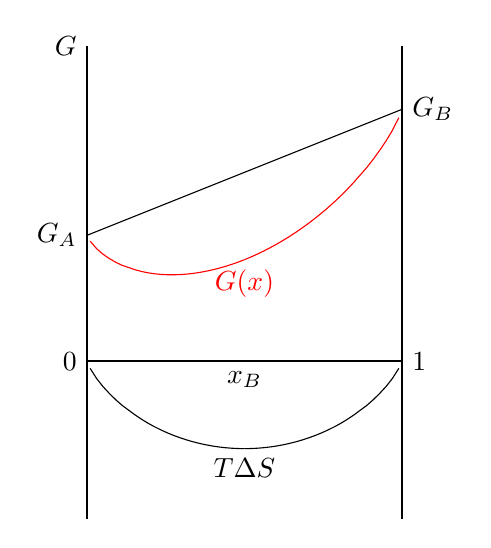
\begin{tikzpicture}[scale=4]
            \draw[thick] (0,0) node[anchor=east]{0} --(0.5,0) node[anchor=north] {$x_B$}--(1,0) node[anchor=west]{1};
            \draw[thick] (0,-0.5) -- (0,0.4) node[anchor=east]{$G_A$}--(0,1) node[anchor=east]{$G$};
            \draw[thick] (1,-0.5) -- (1,0.8) node[anchor=west]{$G_B$}--(1,1);
            
            \draw[thin] (0,0.4)--(1,0.8);
            \draw[domain=0.01:0.5] plot(\x,{0.4*(\x*ln(\x)+(1-\x)*ln((1-\x)))})
                node[below] {$T\Delta S$};
            \draw[domain=0.5:0.99] plot(\x,{0.4*(\x*ln(\x)+(1-\x)*ln((1-\x)))});
            %G(x)
            \draw[red,domain=0.01:0.5] plot(\x,{0.4*\x+0.4+0.4*(\x*ln(\x)+(1-\x)*ln((1-\x)))})
                node[below] {$G(x)$};
            \draw[red,domain=0.5:0.99] plot(\x,{0.4*\x+0.4+0.4*(\x*ln(\x)+(1-\x)*ln((1-\x)))});        
        \end{tikzpicture}
       % \caption{$\Delta H^M=0$,混合时结合能不变的自由能曲线。}
        \label{混合时结合能不变的自由能曲线}
    }
   % \end{subfigure}
   % \begin{subfigure}[0.3\textwidth]
    \subfigure[混合时结合能减小的自由能曲线]
    {
           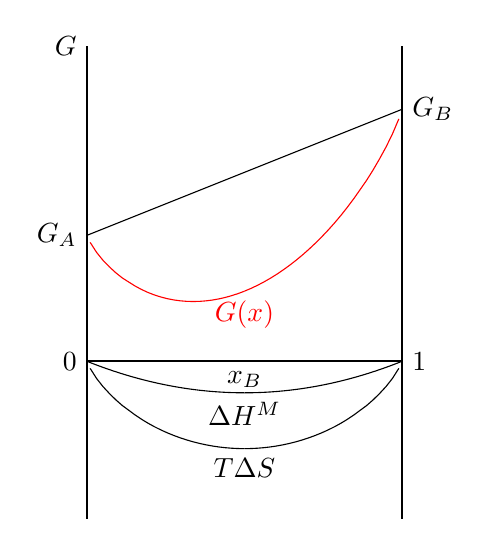
\begin{tikzpicture}[scale=4]
            \draw[thick] (0,0) node[anchor=east]{0} --(0.5,0) node[anchor=north] {$x_B$}--(1,0) node[anchor=west]{1};
            \draw[thick] (0,-0.5) -- (0,0.4) node[anchor=east]{$G_A$}--(0,1) node[anchor=east]{$G$};
            \draw[thick] (1,-0.5) -- (1,0.8) node[anchor=west]{$G_B$}--(1,1);
            %G(0)
            \draw[thin] (0,0.4)--(1,0.8);
            %T\Delta S
            \draw[domain=0.01:0.5] plot(\x,{0.4*(\x*ln(\x)+(1-\x)*ln((1-\x)))})
                node[below] {$T\Delta S$};
            \draw[domain=0.5:0.99] plot(\x,{0.4*(\x*ln(\x)+(1-\x)*ln((1-\x)))});
            %\Delta H
            \draw[domain=0:0.5] plot(\x,{-0.4*(\x*(1-\x))})
                node[below] {$\Delta H^M$};
            \draw[domain=0.5:1] plot(\x,{-0.4*(\x*(1-\x))});
            
            %G(x)
            \draw[red,domain=0.01:0.5] plot(\x,{0.4*\x+0.4-0.4*(\x*(1-\x))+0.4*(\x*ln(\x)+(1-\x)*ln((1-\x)))})
                node[below] {$G(x)$};
            \draw[red,domain=0.5:0.99] plot(\x,{0.4*\x+0.4-0.4*(\x*(1-\x))+0.4*(\x*ln(\x)+(1-\x)*ln((1-\x)))});        
        \end{tikzpicture}
        %\caption{$\Delta H^M<0$,混合时结合能小于零的自由能曲线。}
        \label{混合时结合能减小的自由能曲线}
    }
    
    %\end{subfigure}
    \caption{三种不同情况的自由能曲线}
\end{figure}


                当焓变小于零时,也就是$\Delta H^M<0$,
                \begin{equation}
                    \frac{\partial^{2} G}{\partial x_{B}^{2}}=2 \alpha^{\prime}+R T\left(\frac{1}{x_{A}}+\frac{1}{x_{B}}\right)<0,
                \end{equation}
                这时异类原子的结合力大于同类原子之间的结合力。表现为在溶解时会放出热量。此时$G(x)$为下垂线,曲线的凹陷更大,如\autoref{混合时结合能减小的自由能曲线}所示。

                当焓变大于零时,焓变与熵的变化为相反的作用,曲线的形状与两者的大小有关。
                
                
                \begin{figure}[ht]
    \centering
    %\begin{subfigure}[0.3\textwidth]
    \subfigure[$T>\frac{\alpha^{\prime}}{2R}$]
    {
        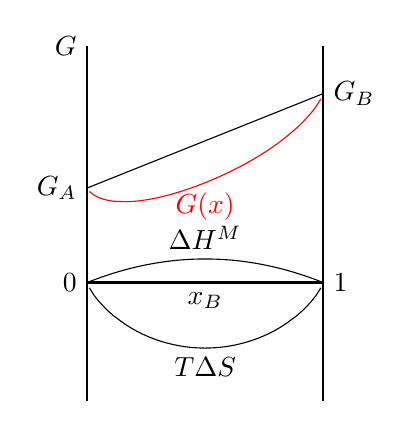
\begin{tikzpicture}[scale=3]
            \draw[thick] (0,0) node[anchor=east]{0} --(0.5,0) node[anchor=north] {$x_B$}--(1,0) node[anchor=west]{1};
            \draw[thick] (0,-0.5) -- (0,0.4) node[anchor=east]{$G_A$}--(0,1) node[anchor=east]{$G$};
            \draw[thick] (1,-0.5) -- (1,0.8) node[anchor=west]{$G_B$}--(1,1);
            
            \draw[thin] (0,0.4)--(1,0.8);
            \draw[domain=0.01:0.5] plot(\x,{0.4*(\x*ln(\x)+(1-\x)*ln((1-\x)))})
                node[below] {$T\Delta S$};
            \draw[domain=0.5:0.99] plot(\x,{0.4*(\x*ln(\x)+(1-\x)*ln((1-\x)))});
            
            %\Delta H
            \draw[domain=0:0.5] plot(\x,{0.4*(\x*(1-\x))})
                node[anchor=south] {$\Delta H^M$};
            \draw[domain=0.5:1] plot(\x,{0.4*(\x*(1-\x))});
            
            %G(x)
            \draw[red,domain=0.01:0.5] plot(\x,{0.4*\x+0.4+0.4*(\x*(1-\x))+0.4*(\x*ln(\x)+(1-\x)*ln((1-\x)))})
                node[below] {$G(x)$};
            \draw[red,domain=0.5:0.99] plot(\x,{0.4*\x+0.4+0.4*(\x*(1-\x))+0.4*(\x*ln(\x)+(1-\x)*ln((1-\x)))});        
        \end{tikzpicture}
       % \caption{$\Delta H^M=0$,混合时结合能不变的自由能曲线。}
        \label{subfig:高温下混合时结合能增加的自由能曲线}
    }
   % \end{subfigure}
   % \begin{subfigure}[0.3\textwidth]
    \subfigure[$0<T<\frac{\alpha^{\prime}}{2R}$]
    {
           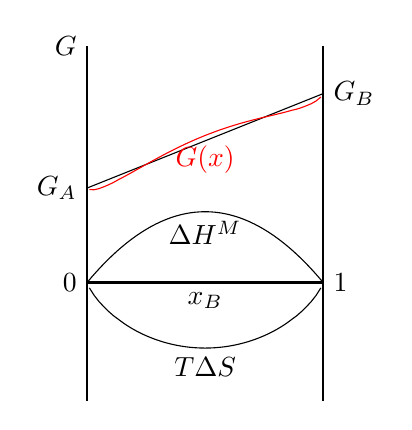
\begin{tikzpicture}[scale=3]
            \draw[thick] (0,0) node[anchor=east]{0} --(0.5,0) node[anchor=north] {$x_B$}--(1,0) node[anchor=west]{1};
            \draw[thick] (0,-0.5) -- (0,0.4) node[anchor=east]{$G_A$}--(0,1) node[anchor=east]{$G$};
            \draw[thick] (1,-0.5) -- (1,0.8) node[anchor=west]{$G_B$}--(1,1);
            %G(0)
            \draw[thin] (0,0.4)--(1,0.8);
            %T\Delta S
            \draw[domain=0.01:0.5] plot(\x,{0.4*(\x*ln(\x)+(1-\x)*ln((1-\x)))})
                node[below] {$T\Delta S$};
            \draw[domain=0.5:0.99] plot(\x,{0.4*(\x*ln(\x)+(1-\x)*ln((1-\x)))});
            %\Delta H
            \draw[domain=0:0.5] plot(\x,{1.2*(\x*(1-\x))})
                node[below] {$\Delta H^M$};
            \draw[domain=0.5:1] plot(\x,{1.2*(\x*(1-\x))});
            
            %G(x)
            \draw[red,domain=0.01:0.5] plot(\x,{0.4*\x+0.4+1.2*(\x*(1-\x))+0.4*(\x*ln(\x)+(1-\x)*ln((1-\x)))})
                node[below] {$G(x)$};
            \draw[red,domain=0.5:0.99] plot(\x,{0.4*\x+0.4+1.2*(\x*(1-\x))+0.4*(\x*ln(\x)+(1-\x)*ln((1-\x)))});        
        \end{tikzpicture}
        %\caption{$\Delta H^M<0$,混合时结合能小于零的自由能曲线。}
        \label{subfig:低温下混合时结合能增加的自由能曲线}
    }
    \subfigure[$T=0$]
    {
        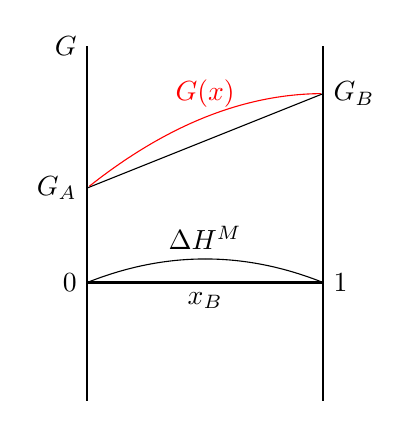
\begin{tikzpicture}[scale=3]
            \draw[thick] (0,0) node[anchor=east]{0} --(0.5,0) node[anchor=north] {$x_B$}--(1,0) node[anchor=west]{1};
            \draw[thick] (0,-0.5) -- (0,0.4) node[anchor=east]{$G_A$}--(0,1) node[anchor=east]{$G$};
            \draw[thick] (1,-0.5) -- (1,0.8) node[anchor=west]{$G_B$}--(1,1);
            %G(0)
            \draw[thin] (0,0.4)--(1,0.8);
            %T\Delta S
            %\draw[domain=0.01:0.5] plot(\x,{0.4*(\x*ln(\x)+(1-\x)*ln((1-\x)))})
            %    node[below] {$T\Delta S$};
            %\draw[domain=0.5:0.99] plot(\x,{0.4*(\x*ln(\x)+(1-\x)*ln((1-\x)))});
            %\Delta H
            \draw[domain=0:0.5] plot(\x,{0.4*(\x*(1-\x))})
                node[anchor=south] {$\Delta H^M$};
            \draw[domain=0.5:1] plot(\x,{0.4*(\x*(1-\x))});
            
            %G(x)
            \draw[red,domain=0.01:0.5] plot(\x,{0.4*\x+0.4+0.4*(\x*(1-\x))})
                node[anchor=south] {$G(x)$};
            \draw[red,domain=0.5:0.99] plot(\x,{0.4*\x+0.4+0.4*(\x*(1-\x))});        
        \end{tikzpicture}
        %\caption{$\Delta H^M<0$,混合时结合能小于零的自由能曲线。}
        \label{subfig:绝对零度下混合时结合能增加的自由能曲线}
    }
    %\end{subfigure}
    \caption{混合时结合能增加的在不同温度下的自由能曲线}

\end{figure}

                
                当$T\geq\frac{\alpha^{\prime}}{2R}$时,混合所提高的内能全部由热温熵来补充,$\Delta G^m\leq0$,曲线仍然为下垂曲线,仅仅是下垂的程度小一点,如\autoref{subfig:高温下混合时结合能增加的自由能曲线}所示。

                在低温情况下,$T<\frac{\alpha^{\prime}}{2R}$时,构成的曲线有三个极值点和两个拐点,在靠近坐标轴($x$接近0或1)处为上凹曲线,有两个极小值,而中部位凹向朝下的上凸曲线,会有一极大值,如\autoref{subfig:低温下混合时结合能增加的自由能曲线}所示。
                在这种情况下,存在两种必然的规律:
                \begin{enumerate}
                    \item[1] 任何一个组元都可以少量溶解其它组元,不可能得到绝对的纯净物质;
                    \item[2] 当出现上凸时,吉布斯自由能会提高,自发的趋势是形成两相混合物可以降低体系的自由能,两组元表现为有限溶解。
                \end{enumerate}
    \section{均匀形核}
        相变动力学\index{相变动力学}是讨论相变的过程和速度的,新相的形核\index{形核}和长大\index{长大}是动力学的两个基本问题。

        即使在宏观的单相均匀系统中,也存在着微观的不均匀性,存在局部的能量、密度、成分组态的涨落。Gibbs将这种涨落分为两类:
        \begin{enumerate}
            \item[1] 在\textbf{很小的体积}内存在着剧烈的原子再分布,在亚稳的母相中形成\textbf{新相胚芽},当这种胚芽超过临界尺寸\index{形核!临界尺寸},就变成稳定的新相核心而自发长大,金属和合金中的转变多数如此;
            \item[2] 在\textbf{大的体积内}原子的少量调整,\textbf{转变在整个体积范围内进行},如有序-无序转变\index{有序-无序转变}。
        \end{enumerate}

        以纯金属的凝固为例,假设在$L$中形成半径为$r$的晶核\index{形核!晶核}$s$,固体和液体的体积为$V_s$和$V_L$,固体和液体单位体积的自由能为$G_v^s$、$G_v^L$,$A_{SL}$为两相之间面积,$r_{SL}$为两相的界面能。

        假设发生相变的过程中没有体积变化,没有形核时,体系的自由能为
        \begin{equation}
            G_1=\left( V_s+V_l \right)G_v^L,
        \end{equation}
        则体系中出现晶核的自由能为:
        \begin{equation}
            G_2=V_sG_v^S+V_LG_v^L+A_{SL}\gamma_{SL},
        \end{equation}
        所以形核时的自由能变化为
        \begin{equation}
            \Delta G_v=G_2-G_1=-V_S\cdot \Delta G_v++A_{SL}\gamma_{SL},
        \end{equation}
        式中$\Delta G_v=G_v^L-G_v^S$。
        
        假设晶核为球形,则固液界面面积和固体体积为
        \begin{equation}
            A_{SL}=4\pi r^2, V=\frac{4}{3}\pi r^3,
        \end{equation}
        形核的自由能变化量为
        \begin{equation}
            \Delta G_r=-\frac{4}{3}\pi r^3\Delta G_v+4\pi r^2\gamma_{SL},
        \end{equation}
        在平衡状态下,对$r$求导,
        \begin{equation}
            \frac{\dif \Delta G_r }{\dif r}=-4\pi r^2\Delta G_v+8\pi r\gamma_{SL},
        \end{equation}
        令导数为零,此时的晶核半径为临界晶核尺寸\index{临界晶核尺寸}
        \begin{equation}
            r^*=\frac{\gamma_{SL}}{\Delta G_v}.
        \end{equation}
        自由能改变量为
        \begin{equation}
            \Delta G^*=\frac{16\pi}{3}\left( \frac{\gamma_{SL}^3}{\Delta G_v^2} \right),
        \end{equation}
        根据自由能的二阶导数可知,此时的自由能为极大值。因此只有半径大于临界晶核尺寸的晶核才能继续长大,而小于该尺寸的晶核则消失。
        临界晶核对于的自由能变化量$\Delta G^*$为形核功,即核长大到$r^*$所需克服的势垒。

        形核功的量值是临界球形晶核表面能的$1/3$,也就是说,球形晶核的表面能的$2/3$由新相的自由能下降给出,
        $1/3$依靠热涨落。这一过程称为\textbf{热激活过程}\index{形核!热激活过程}。

        在凝固过程中,要达到临界半径,需要温度上提供足够的过冷度,假设熔点温度为$T_m$,外界温度与熔点温度差为$\Delta T$,
        此时的自由能变化量为
        \begin{equation}
            \Delta G_v=\frac{\Delta T\cdot\Delta H_m}{T_m},
        \end{equation}
        代入临界半径表达式为
        \begin{equation}
            r^*=\frac{2\gamma_{LS}T_m}{\Delta H_m\cdot\Delta T},
        \end{equation}
        因此当$\Delta T=0$,$\Delta G^*\to0$,不能形核,过冷度越大,越易形核。
    \section{形核速率及均匀形核在固态转变中的推广}
        在液态的情况下,金属中也会存在一些小区域具有固态的密堆结构,本章将对这些小区域进行讨论。

        假设在单位体积内,由$i$个分子组成半径为$r$的胚芽数为$n_i$,而单分子数目为$n$,
        而单位体积中独立质点数$N$为
        \begin{equation}
            N=n+\sum_{i\geq2}n_i,
        \end{equation}
        由于$\sum_{i\geq2}n_i\ll n$,所以$N$约等于单位体积中的分子数。从统计方面考虑,胚芽数$n_i$服从玻尔兹曼分布:
        \begin{equation}
            n_i=N e^{-\frac{\Delta G_r}{kT}},
        \end{equation}
        临界核心数$n_i^*$为
        \begin{equation}
            n_i^*=N e^{-\frac{\Delta G_r^*}{kT}},
        \end{equation}
        其中$\Delta G_r^*$为形核功。

        在临界核心上痛殴分子碰撞再增加一个分子,它就可以克服势垒称为稳定的新相核心。
        定义单位体积中单位时间内形成的新相稳定核心的数目为形核速率\index{形核速率}$I$,
        所以形核速率$I$正比于临近核心的分子加入核心的频率$\omega$,即
        \begin{equation}
            I=\omega\cdot n_i^*=\omega N e^{-\frac{\Delta G_r^*}{kT}}\label{形核速率},
        \end{equation}
        $\omega$取决于原子振动频率、扩散激活能、晶核的表面积等。

        \subsection{形核引起的晶格畸变}
            在金属相变的过程中,由于晶核周围的体积和形状可能发生变
            化,或者晶核受到周围晶格的限制,使得晶核中的原子不能处
            在平衡位置,这两种情况都消耗弹性应变能$\varepsilon$,这种弹性应变
            能通过扩散和范性流变才能松弛。

            假定应变能正比于晶核的体积,则形核的自由能写作
            \begin{equation}
                \Delta G_r=-\frac{4}{3}\pi \cdot r^3(\Delta G_v+\varepsilon)+4\pi\cdot r^2\cdot\gamma_{SL},
            \end{equation}
            临界半径变为
            \begin{equation}
                r^*=\frac{2\gamma_{SL}}{\Delta G_v+\varepsilon},
            \end{equation}
            形核功为
            \begin{equation}
                \Delta G^*=\frac{16\pi \gamma^3_{SL}}{3(\Delta G_v+\varepsilon)^2}.
            \end{equation}
            另外,假设晶核的表面积对此时的邻近核心的分子加入核心的频率$\omega$没有影响,可以写为
            \begin{equation}
                \omega=ve^{-\frac{\Delta G_m}{kT}},
            \end{equation}
            其中$v$是原子振动频率\index{形核速率!原子振动频率},$\Delta G_m$是原子扩散的激活能\index{形核速率!扩散激活能}。所以\autoref{形核速率}可以写为
            \begin{equation}
                I=Nve^{-\frac{\Delta G^*+\Delta G_m}{kT}}\label{考虑外来扩散原子的形核速率},
            \end{equation}
            式中,$Nv$对$I$的影响很小,形核速率强烈依赖指数因子,也就是形核功和原子扩散激活能。
            对于固态相变,合理的数量级为
            \begin{equation*}
                Nve^{-\frac{\Delta G_m}{kT}}\simeq 10^{30},I=10^{30}e^{-\frac{\Delta G^*}{kT}}.
            \end{equation*}

            由于$\Delta G^*$因过冷度$\Delta T$的增大而减小,所以\textbf{形核速率强烈依赖于温度}。
            当$\Delta T\to0$,$\Delta G^*\to\infty$,$I\to0$,$\Delta T$增大,形核速率$I$存在极值,
            先增大后减小。

            \begin{figure}[ht]
                \centering
                    \subfigure[某合金的局部相图。]
                    {
                        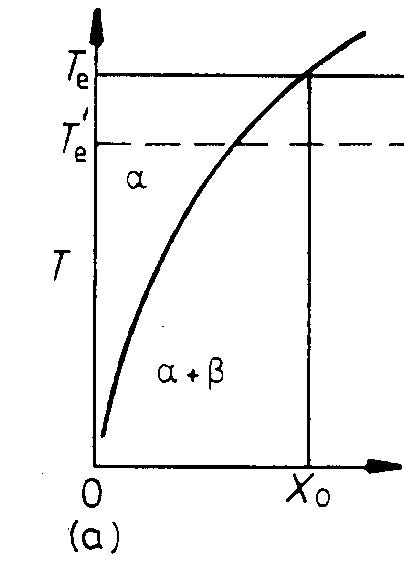
\includegraphics{fig/均匀形核速率I与转变温度之间的关系/a.jpg}
                        \label{subfigure:某合金的局部相图}
                    }
                    \subfigure[相图的有效推动能量与形核功与转变温度之间的关系。]
                    {
                        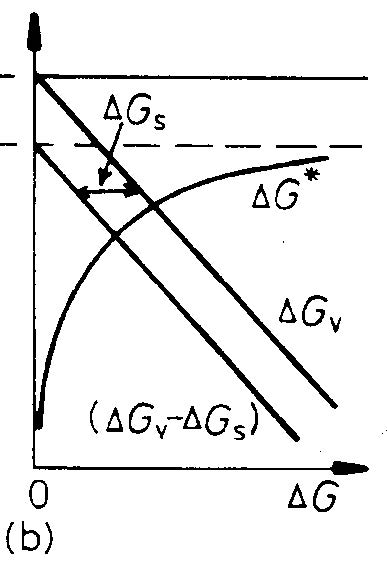
\includegraphics{fig/均匀形核速率I与转变温度之间的关系/b.jpg}
                    }
                    \\
                    \subfigure[确定$I$的两个指数项与温度的关系。]
                    {
                        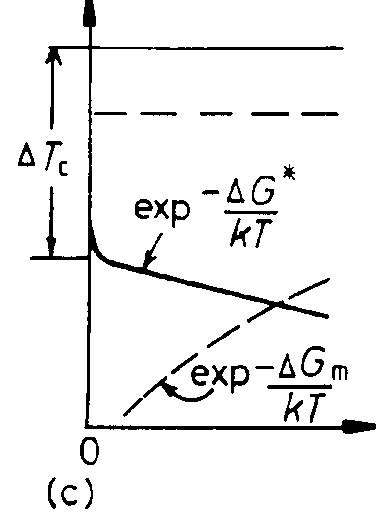
\includegraphics{fig/均匀形核速率I与转变温度之间的关系/c.jpg}
                    }
                    \subfigure[$I $随温度的变化。]
                    {
                        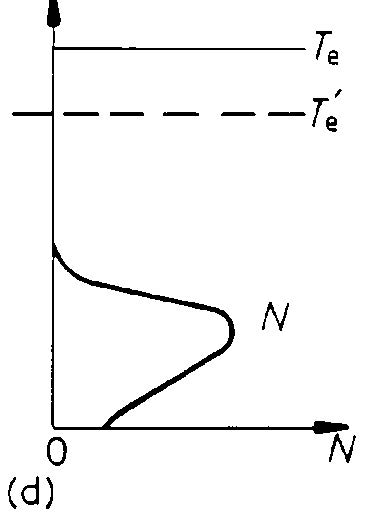
\includegraphics{fig/均匀形核速率I与转变温度之间的关系/d.jpg}
                        \label{subfigure:$I $随温度的变化}
                    }
                \caption{均匀形核速率$I$与转变温度之间的关系。}
                \label{均匀形核速率I与转变温度之间的关系}
            \end{figure}

            从\autoref{subfigure:某合金的局部相图}可知,成分为$x_0$的合金,其固溶温度为$T_e$,为了抵消应变能$\Delta G_\varepsilon$,
            必须过冷到$T_e^{\prime}$才能析出第二相$\beta$。形核速率随$T$的变化如\autoref{subfigure:$I $随温度的变化}所示,
            在高温下,沉淀的推动能量很小,因为$\Delta G^*$很大,所以$I$很小;在低温情况下,由于扩散很慢,所以$I$也很小,在中间某一个温度,
            $I$有极大值。

        \subsection{相界面性质的影响}

            界面能\index{界面能}$\gamma$的来源可以分为两部分,
            \begin{itemize}
                \item[1] 一部分是在母相中形成新相界面时,同类键和异类键的数量变化引起的,称为界面能中的\textbf{化学项}\index{界面能!化学项};
                \item[2] 另一部分是界面结构引起的 (如界面上产生的位错),称为界面能中的\textbf{结构项}\index{界面能!结构项}。
            \end{itemize}
            
            如果新相和母相的晶体结构和取向相同,电阵常数也非常接近,形成\textbf{完全共格界面}\index{完全共格界面}。界面能
            较小,只包括化学项,结构项(畸变能$\varepsilon$)趋于0,长大速度很快。

            如果完全共格两相的点阵常数不同,就会在界面上引入位错,来减少界面能中的体积应变能,结构项略有增大,形成\textbf{部分共格界面}\index{部分共格界面}。

            若新相通过母相切变形成,某些界面点阵相似,这种界面称为\textbf{切变共格}\index{切变共格}。

            如果所有界面都不共格,称为\textbf{非共格}\index{非共格}新相。

            
    \section{非均匀形核(界面形核)}
        
    \section{过饱和固溶体的脱溶沉淀}
    \section{调幅分解}
    \section{马氏体相变}
\part{考试内容}
	\chapter{晶体缺陷}
    \section{问题}
    \begin{itemize}
        \item[1] 从几何形态上说,晶体缺陷分哪几类,试举几个典型例子,位错与空位之间有何相互作用?
        \item[2] 为何为点缺陷的形成能和迁移能,为什么说点缺陷是一种热力学平衡缺陷?一定温度下空位平衡浓度的表达式是什么,有什么特点?
        \item[3] 什么叫非平衡点缺陷?试举例说明它的产生方法?
        \item[4] 什么叫位错,位错密度的表达式是什么?
        \item[5] 试总结与比较刃型,螺型及混合位错下列方面的异同(从结构类型,柏式矢量,应力场特点,应变能和张力方面进行描述)。
        \item[6] 何谓柏格斯矢量,柏氏矢量的特点及确定方法。单位长位错的应变能及张力近似表达式是什么?
        \item[7] 为何要引入位错的点阵模型,它能说明什么问题。什么叫位错线宽度,位错中心能量?定性叙述位错的 Pelels模型。
        \item[8] 计算位错运动引起的变形及位错引起的晶体弯曲?
        \item[9] 什么叫作用在位错上的力,这力的大小,方向及特点是什么(分别讨论滑移力,攀移力,化学力),位错受力的 peach公式及由此计算位错在应力场中受到的滑移和攀移力。 
        \item[10] 分类叙述不同类型平行位错线间相互作用力大小,方向及特点?何为位错塞积?
        \item[11] 不同的两条位错相遇时会发生哪些现象?位错反应发生的基本条件是什么?
        \item[12] 不同面位错相互切割后会在各位错线上造成什么后果?什么叫割阶以及它们的运动方式?
        \item[13] 试述位错FR源的动作原理及动作应力表达式?
        \item[14] 什么叫层错?简述面心立方晶体中的不全位错(半,偏位错),扩展位错?什么叫全位错和不动位错?试比较全位错和不全位错的异同点。
        \item[15] 为何说晶界有5个自由度,什么叫扭转晶界,倾转晶界及亚品界?
        \item[16] 晶界为何具有能量,近代关于晶界结构的基本看法是什么?
    \end{itemize}
\printindex
\end{document}
